% Thesis hero, two-pole PHOTO collage (P1 analog: fig_corpus_collage / p1_fig1).
% AUTO-GENERATED by no_upload/gen_collage_p3.py. Tiles are real figures harvested from
% each benchmark's arXiv paper; per-tile provenance in Table~\ref{tab:collage_provenance}.
\begin{figure*}[tp]
\centering
\resizebox{\textwidth}{!}{%
\begin{tikzpicture}[x=1cm,y=1cm]
\fill[black!88] (0,0) rectangle (13.80,-0.72);
\node[anchor=west,text=white,font=\large\bfseries,inner sep=0] at (0.16,-0.36) {Predict or Act?};
\node[anchor=east,text=white!70,font=\scriptsize,inner sep=0] at (13.64,-0.36) {the benchmark landscape on one axis; each tile links to its paper};
\fill[cat-vla!70!black] (0,-0.72) rectangle (5.55,-1.22);
\node[anchor=west,text=white,font=\footnotesize,inner sep=0] at (0.12,-0.97) {{\bfseries CLOSED-LOOP}\, task-success suites};
\fill[cat-skill!70!black] (8.25,-0.72) rectangle (13.80,-1.22);
\node[anchor=west,text=white,font=\footnotesize,inner sep=0] at (8.37,-0.97) {{\bfseries OPEN-LOOP}\, world-model \& video eval};
\fill[black!5] (5.55,-0.72) rectangle (8.25,-6.55);
\draw[black!25,line width=0.4pt] (5.55,-0.72)--(5.55,-6.55);
\draw[black!25,line width=0.4pt] (8.25,-0.72)--(8.25,-6.55);
\node[text=black,font=\small\bfseries,align=center,inner sep=0] at (6.90,-1.95) {what does it\\ score?};
\node[text=black!70,font=\scriptsize,align=center,inner sep=0] at (6.90,-2.85) {$\leftarrow$ task success\\ (closed loop)};
\node[text=black,font=\Large\bfseries,inner sep=0] at (6.90,-3.60) {vs};
\node[text=black!70,font=\scriptsize,align=center,inner sep=0] at (6.90,-4.35) {prediction quality\\ (open loop) $\rightarrow$};
\node[text=black!55,font=\scriptsize\itshape,align=center,text width=2.4cm,inner sep=0] at (6.90,-5.15) {the survey's organising axis};
\node[text=BrickRed!85!black,font=\scriptsize\bfseries,align=center,text width=2.5cm,inner sep=0] at (6.90,-6.05) {only 11 of 160 test if prediction helps action};
\node[anchor=north west,inner sep=0] at (0.000,-1.280) {\href{https://arxiv.org/abs/2306.03310}{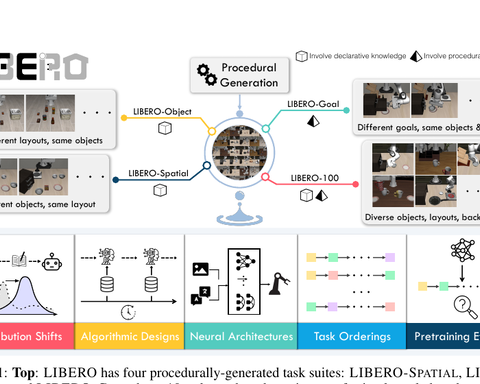
\includegraphics[width=1.803cm,height=1.402cm]{figures/img/collage_tiles/libero.png}}};
\draw[black!35,line width=0.35pt] (0.000,-1.280) rectangle (1.803,-2.682);
\node[anchor=north west,text=ACMDarkBlue,font=\tiny,inner sep=0] at (0.030,-2.702) {\href{https://arxiv.org/abs/2306.03310}{LIBERO}};
\node[anchor=north west,inner sep=0] at (1.873,-1.280) {\href{https://arxiv.org/abs/2112.03227}{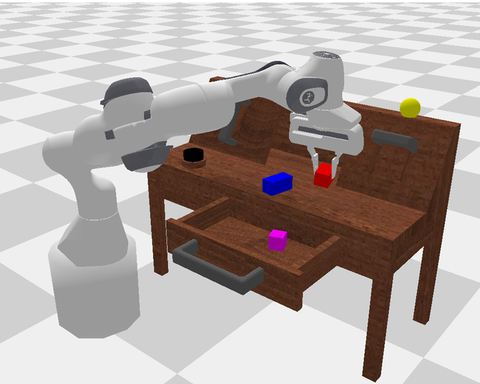
\includegraphics[width=1.803cm,height=1.402cm]{figures/img/collage_tiles/calvin.png}}};
\draw[black!35,line width=0.35pt] (1.873,-1.280) rectangle (3.676,-2.682);
\node[anchor=north west,text=ACMDarkBlue,font=\tiny,inner sep=0] at (1.903,-2.702) {\href{https://arxiv.org/abs/2112.03227}{CALVIN}};
\node[anchor=north west,inner sep=0] at (3.747,-1.280) {\href{https://arxiv.org/abs/1910.10897}{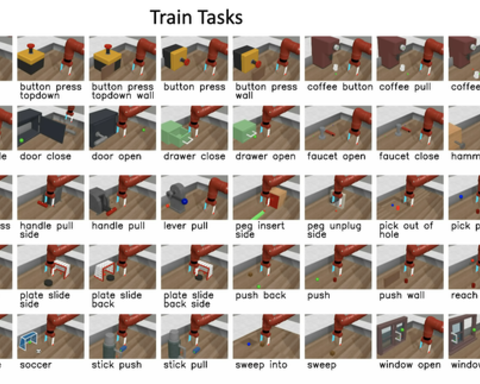
\includegraphics[width=1.803cm,height=1.402cm]{figures/img/collage_tiles/metaworld.png}}};
\draw[black!35,line width=0.35pt] (3.747,-1.280) rectangle (5.550,-2.682);
\node[anchor=north west,text=ACMDarkBlue,font=\tiny,inner sep=0] at (3.777,-2.702) {\href{https://arxiv.org/abs/1910.10897}{Meta-World}};
\node[anchor=north west,inner sep=0] at (0.000,-3.057) {\href{https://arxiv.org/abs/2302.04659}{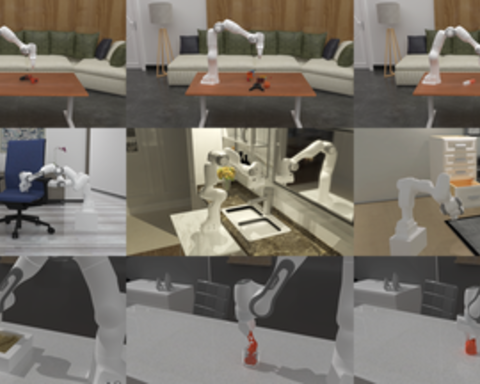
\includegraphics[width=1.803cm,height=1.402cm]{figures/img/collage_tiles/maniskill2.png}}};
\draw[black!35,line width=0.35pt] (0.000,-3.057) rectangle (1.803,-4.459);
\node[anchor=north west,text=ACMDarkBlue,font=\tiny,inner sep=0] at (0.030,-4.479) {\href{https://arxiv.org/abs/2302.04659}{ManiSkill2}};
\node[anchor=north west,inner sep=0] at (1.873,-3.057) {\href{https://arxiv.org/abs/2406.02523}{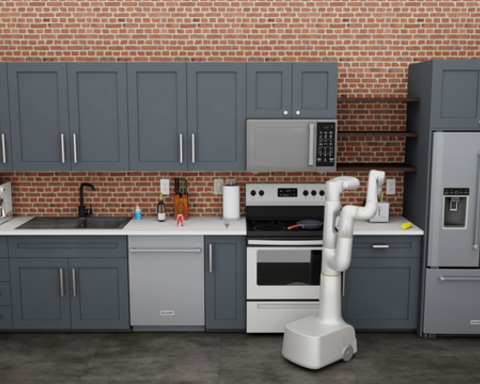
\includegraphics[width=1.803cm,height=1.402cm]{figures/img/collage_tiles/robocasa.png}}};
\draw[black!35,line width=0.35pt] (1.873,-3.057) rectangle (3.676,-4.459);
\node[anchor=north west,text=ACMDarkBlue,font=\tiny,inner sep=0] at (1.903,-4.479) {\href{https://arxiv.org/abs/2406.02523}{RoboCasa}};
\node[anchor=north west,inner sep=0] at (3.747,-3.057) {\href{https://arxiv.org/abs/2310.13724}{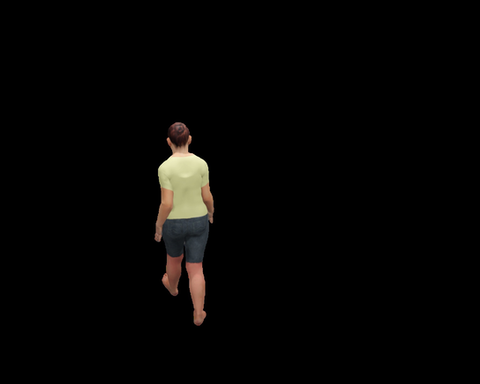
\includegraphics[width=1.803cm,height=1.402cm]{figures/img/collage_tiles/habitat30.png}}};
\draw[black!35,line width=0.35pt] (3.747,-3.057) rectangle (5.550,-4.459);
\node[anchor=north west,text=ACMDarkBlue,font=\tiny,inner sep=0] at (3.777,-4.479) {\href{https://arxiv.org/abs/2310.13724}{Habitat 3.0}};
\node[anchor=north west,inner sep=0] at (0.000,-4.833) {\href{https://arxiv.org/abs/1912.01734}{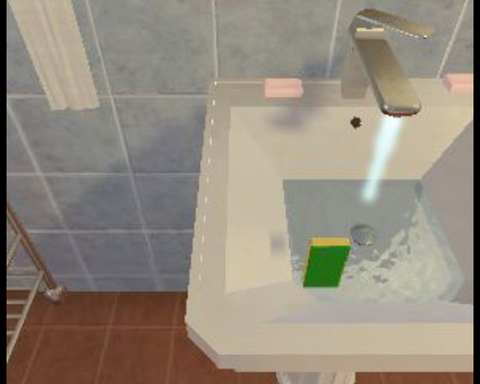
\includegraphics[width=1.803cm,height=1.402cm]{figures/img/collage_tiles/alfred.png}}};
\draw[black!35,line width=0.35pt] (0.000,-4.833) rectangle (1.803,-6.235);
\node[anchor=north west,text=ACMDarkBlue,font=\tiny,inner sep=0] at (0.030,-6.255) {\href{https://arxiv.org/abs/1912.01734}{ALFRED}};
\node[anchor=north west,inner sep=0] at (1.873,-4.833) {\href{https://arxiv.org/abs/2410.01345}{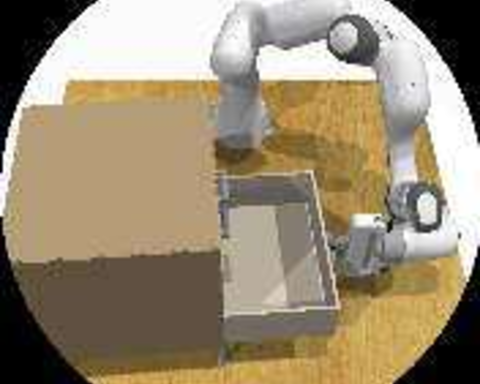
\includegraphics[width=1.803cm,height=1.402cm]{figures/img/collage_tiles/gembench.png}}};
\draw[black!35,line width=0.35pt] (1.873,-4.833) rectangle (3.676,-6.235);
\node[anchor=north west,text=ACMDarkBlue,font=\tiny,inner sep=0] at (1.903,-6.255) {\href{https://arxiv.org/abs/2410.01345}{GemBench}};
\node[anchor=north west,inner sep=0] at (3.747,-4.833) {\href{https://arxiv.org/abs/2412.18194}{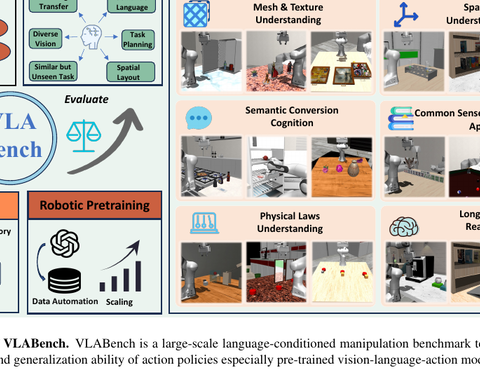
\includegraphics[width=1.803cm,height=1.402cm]{figures/img/collage_tiles/vlabench.png}}};
\draw[black!35,line width=0.35pt] (3.747,-4.833) rectangle (5.550,-6.235);
\node[anchor=north west,text=ACMDarkBlue,font=\tiny,inner sep=0] at (3.777,-6.255) {\href{https://arxiv.org/abs/2412.18194}{VLABench}};
\node[anchor=north west,inner sep=0] at (8.250,-1.280) {\href{https://arxiv.org/abs/2502.20694}{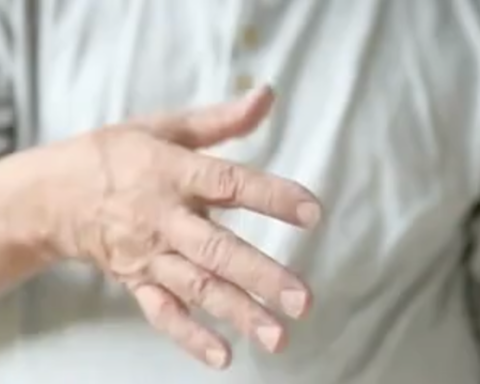
\includegraphics[width=1.803cm,height=1.402cm]{figures/img/collage_tiles/worldmodelbench.png}}};
\draw[black!35,line width=0.35pt] (8.250,-1.280) rectangle (10.053,-2.682);
\node[anchor=north west,text=ACMDarkBlue,font=\tiny,inner sep=0] at (8.280,-2.702) {\href{https://arxiv.org/abs/2502.20694}{WorldModelBench}};
\node[anchor=north west,inner sep=0] at (10.123,-1.280) {\href{https://arxiv.org/abs/2501.09038}{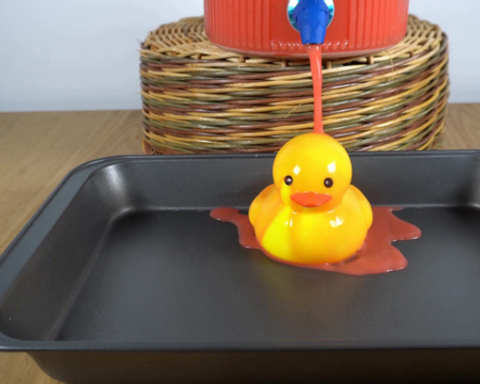
\includegraphics[width=1.803cm,height=1.402cm]{figures/img/collage_tiles/physicsiq.png}}};
\draw[black!35,line width=0.35pt] (10.123,-1.280) rectangle (11.926,-2.682);
\node[anchor=north west,text=ACMDarkBlue,font=\tiny,inner sep=0] at (10.153,-2.702) {\href{https://arxiv.org/abs/2501.09038}{Physics-IQ}};
\node[anchor=north west,inner sep=0] at (11.997,-1.280) {\href{https://arxiv.org/abs/2504.00983}{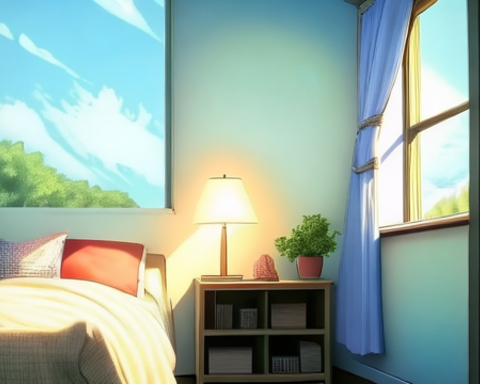
\includegraphics[width=1.803cm,height=1.402cm]{figures/img/collage_tiles/worldscore.png}}};
\draw[black!35,line width=0.35pt] (11.997,-1.280) rectangle (13.800,-2.682);
\node[anchor=north west,text=ACMDarkBlue,font=\tiny,inner sep=0] at (12.027,-2.702) {\href{https://arxiv.org/abs/2504.00983}{WorldScore}};
\node[anchor=north west,inner sep=0] at (8.250,-3.057) {\href{https://arxiv.org/abs/2505.09694}{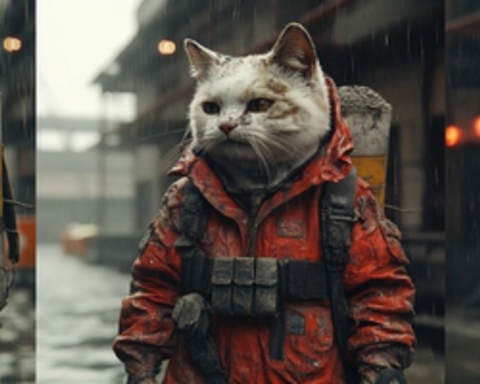
\includegraphics[width=1.803cm,height=1.402cm]{figures/img/collage_tiles/ewmbench.png}}};
\draw[black!35,line width=0.35pt] (8.250,-3.057) rectangle (10.053,-4.459);
\node[anchor=north west,text=ACMDarkBlue,font=\tiny,inner sep=0] at (8.280,-4.479) {\href{https://arxiv.org/abs/2505.09694}{EWMBench}};
\node[anchor=north west,inner sep=0] at (10.123,-3.057) {\href{https://arxiv.org/abs/2410.15461}{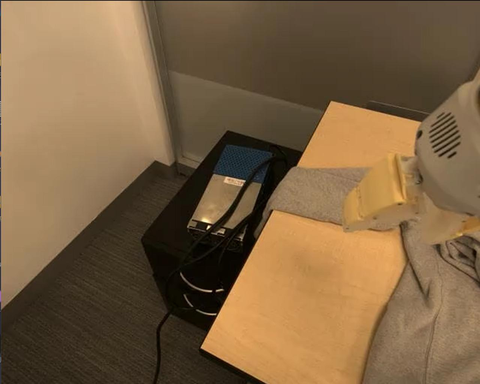
\includegraphics[width=1.803cm,height=1.402cm]{figures/img/collage_tiles/evabench.png}}};
\draw[black!35,line width=0.35pt] (10.123,-3.057) rectangle (11.926,-4.459);
\node[anchor=north west,text=ACMDarkBlue,font=\tiny,inner sep=0] at (10.153,-4.479) {\href{https://arxiv.org/abs/2410.15461}{EVA-Bench}};
\node[anchor=north west,inner sep=0] at (11.997,-3.057) {\href{https://arxiv.org/abs/2406.03520}{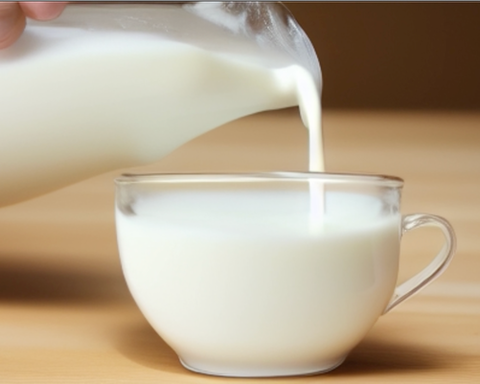
\includegraphics[width=1.803cm,height=1.402cm]{figures/img/collage_tiles/videophy.png}}};
\draw[black!35,line width=0.35pt] (11.997,-3.057) rectangle (13.800,-4.459);
\node[anchor=north west,text=ACMDarkBlue,font=\tiny,inner sep=0] at (12.027,-4.479) {\href{https://arxiv.org/abs/2406.03520}{VideoPhy}};
\node[anchor=north west,inner sep=0] at (8.250,-4.833) {\href{https://arxiv.org/abs/2306.15668}{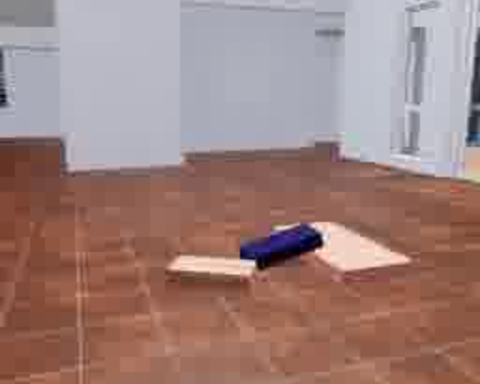
\includegraphics[width=1.803cm,height=1.402cm]{figures/img/collage_tiles/physionpp.png}}};
\draw[black!35,line width=0.35pt] (8.250,-4.833) rectangle (10.053,-6.235);
\node[anchor=north west,text=ACMDarkBlue,font=\tiny,inner sep=0] at (8.280,-6.255) {\href{https://arxiv.org/abs/2306.15668}{Physion++}};
\node[anchor=north west,inner sep=0] at (10.123,-4.833) {\href{https://arxiv.org/abs/2106.08261}{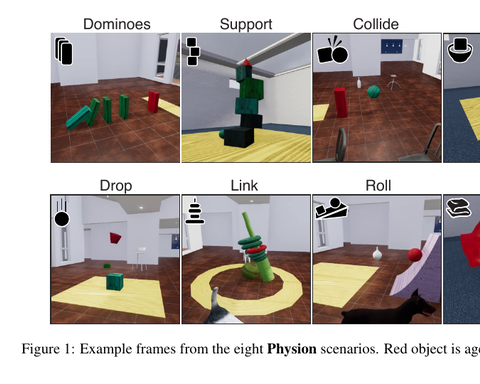
\includegraphics[width=1.803cm,height=1.402cm]{figures/img/collage_tiles/physion.png}}};
\draw[black!35,line width=0.35pt] (10.123,-4.833) rectangle (11.926,-6.235);
\node[anchor=north west,text=ACMDarkBlue,font=\tiny,inner sep=0] at (10.153,-6.255) {\href{https://arxiv.org/abs/2106.08261}{Physion}};
\node[anchor=north west,inner sep=0] at (11.997,-4.833) {\href{https://arxiv.org/abs/2310.11440}{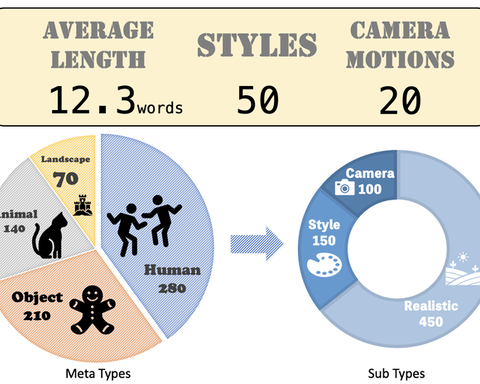
\includegraphics[width=1.803cm,height=1.402cm]{figures/img/collage_tiles/evalcrafter.png}}};
\draw[black!35,line width=0.35pt] (11.997,-4.833) rectangle (13.800,-6.235);
\node[anchor=north west,text=ACMDarkBlue,font=\tiny,inner sep=0] at (12.027,-6.255) {\href{https://arxiv.org/abs/2310.11440}{EvalCrafter}};
\end{tikzpicture}}
\caption{\textbf{Predict or Act?} The survey's organising question, posed with real benchmarks. \emph{Closed-loop} (left): policy and embodied suites score task success by running a policy in the environment. \emph{Open-loop} (right): world-model and video-generation benchmarks score prediction or generation quality with no action. The centre axis is the question neither pole answers, whether prediction earns a closed-loop advantage, built explicitly by only 11 of 160 benchmarks (Table~\ref{tab:landscape}). Every tile is a representative figure from the benchmark's paper and links to it; per-tile provenance is in Table~\ref{tab:collage_provenance}. Images \textcopyright\ their respective authors, reproduced for scholarly review.}
\Description{A two-pole collage of benchmark figures. A black title bar reads ``Predict or Act?''. The left band, CLOSED-LOOP, shows nine policy and embodied benchmark figures; the right band, OPEN-LOOP, shows nine world-model and video-generation benchmark figures; a centre spine contrasts task success (closed loop) with prediction quality (open loop) and notes that only 11 of 160 build the contrast.}
\label{fig:corpus_collage}
\end{figure*}
